%start preamble
\documentclass[paper=a4,fontsize=11pt]{scrartcl}%kind of doc, font size, paper size

\usepackage{fontspec}
\defaultfontfeatures{Ligatures=TeX}
%\setsansfont{Liberation Sans}
\usepackage{polyglossia}	
\setdefaultlanguage[spelling=new, babelshorthands=true]{german}

\usepackage{amsmath}%get math done
\usepackage{graphicx}%get pictures & graphics done
\graphicspath{{pictures/}}%folder to stash all kind of pictures etc
\usepackage{amssymb}%symbolics for math
\usepackage{amsfonts}%extra fonts
\usepackage{caption}%captions under everything
\usepackage{listings}
\usepackage[titletoc]{appendix}
\usepackage[printonlyused,withpage]{acronym}%how to handle acronyms
\usepackage{float}%for garphics and how to let them floating around in the doc
\usepackage{xcolor}%nicer colors, here used for links
\usepackage{wrapfig}%making graphics floated by text and not done by minipage
\usepackage{dsfont}
\usepackage{geometry}
\usepackage{hyperref}
\usepackage{fancyhdr}
\usepackage{multicol}
\usepackage{tasks}
\usepackage{csquotes}

%settings colors for links
\hypersetup{
    colorlinks,
    linkcolor={blue!50!black},
    citecolor={blue},
    urlcolor={blue!80!black}
}

\definecolor{pblue}{rgb}{0.13,0.13,1}
\definecolor{pgreen}{rgb}{0,0.5,0}
\definecolor{pred}{rgb}{0.9,0,0}
\definecolor{pgrey}{rgb}{0.46,0.45,0.48}

%Header & Footers
\pagestyle{fancy}
\lhead{Netzwerke -- Übung\\Sommersemester 2021}
\rhead{FB 4 -- Angewandte Informatik\\Hochschule für Technik und Wirtschft Berlin}
\lfoot{Übungsblatt 04 -- Routing \& Traffic Analysis}
\cfoot{}
\fancyfoot[R]{\thepage}
\renewcommand{\headrulewidth}{0.4pt}
\renewcommand{\footrulewidth}{0.4pt}


\lstdefinestyle{Bash}{
  language=bash,
  showstringspaces=false,
  basicstyle=\small\sffamily,
  numbers=left,
  numberstyle=\tiny,
  numbersep=5pt,
  frame=trlb,
  columns=fullflexible,
  backgroundcolor=\color{gray!20},
  %linewidth=0.9\linewidth,
  %xleftmargin=0.5\linewidth
}

%%here begins the actual document%%
\newcommand{\horrule}[1]{\rule{\linewidth}{#1}} % Create horizontal rule command with 1 argument of height

\DeclareMathOperator{\id}{id}

\begin{document}
\begin{center}
\Large{\textbf{Übungsblatt 04 -- Routing \& Traffic Analysis}}\\
\end{center}

Im Moodle-Kurs liegt eine Zip-Datei \path{network_packets.zip}. Diese enthält verschiedene Dateien die sie auf verschiedene Arten in Wireshark öffnen können. Sie sollen diese Pakete analysieren. Teilweise sind in diesen Paketen Passwörter und Zugangsdaten zu finden, in einigen Fällen können ganze Nachrichten oder Geräteinformationen gefunden werden.

\begin{center}\Large{\textbf{Aufgabe A -- Link Layer \& Ethernet Frames}}\end{center}\vskip0.2in
Das OSI-Modell ordnet verschiedene Funktionalitäten der Netzwerkkommunikation den Schichten des Modells zu. In der untersten Schicht werden physikalische Signale über ein Medium übertragen (bspw. Lichtquanten oder Elektronen). D.h. die Schicht 1 interpretiert direkt die Signale und ermöglicht es Signale in Daten umzuwandeln. Direkt darüber können diese Daten bereits \enquote{höherwertig} verarbeitet werden. Auf dem Link-Layer werden die codierten Daten in Rahmen zusammengefasst. Eigentlich sind die hier transportierten Rahmen nur aneinanderreihungen von Einsen und Nullen.
\begin{enumerate}
	\item Starten sie Wireshark und stellen sie als Adapter \emph{em0} mit Ethernet als Protokoll ein. Erzeugen sie beliebigen Netzwerkverkehr (bspw. Ping auf die eigene IP-Adresse).
	\item Analysieren sie ein Ethernet-Frame unter folgenden Aspekten (Sie können Abb. \ref{ehternet1} als Hilfe nutzen). Skizzieren/notieren sie sich wo und welche Informationen ihres Ethernet-Frames zu finden sind.
	\begin{enumerate}
		\item Welche Größe haben:
		\begin{enumerate}
			\item Wie groß ist ein \emph{IEEE Packet?}
			\item Wie groß ein Ethernet-Frame?
			\item Wie groß ist die eigentliche Nutzlast (Payload/ MAC Client Data)?
		\end{enumerate}
		\item Welchen Zweck hat die Preamble und das \emph{SFD}-Feld?
		\item Wie viele und welche Adressen sind in einem Ethernet-Frame vermerkt?
		\item In Abb. \ref{ehternet1} gibt es innerhalb der Payload ein Feld namens Pad. Wozu dient dies?
		\item Wozu dient die Prüfsumme eines Ethernet-Frames? Wo ist diese zu finden? 
	\end{enumerate}
	\begin{figure}[H]
		\centering
		\includegraphics[scale=0.5]{ethernet1}
		\caption{Aufbau eines Ethernet-Pakets.}
		\label{ehternet1}
		\end{figure}
		\item Wenn ein Ethernet-Frame mitgeschnitten wird, erfolgt dies im Betriebssystem häufig als Hexadezimalzeichen. Diese Datei ist im ZIP-Archiv als \path{raw_ethernet_frame} hinterlegt. Importieren sie die Datei als Hex-Dump in Wireshark.
		\begin{lstlisting}[style=Bash, language=Bash]
0000 00 05 73 a0 00 00 e0 69 95 d8 5a 13 86 dd 60 00
0010 00 00 00 9b 06 40 26 07 53 00 00 60 2a bc 00 00
0020 00 00 ba de c0 de 20 01 41 d0 00 02 42 33 00 00
0030 00 00 00 00 00 04 96 74 00 50 bc ea 7d b8 00 c1
0040 d7 03 80 18 00 e1 cf a0 00 00 01 01 08 0a 09 3e
0050 69 b9 17 a1 7e d3 47 45 54 20 2f 20 48 54 54 50
0060 2f 31 2e 31 0d 0a 41 75 74 68 6f 72 69 7a 61 74
0070 69 6f 6e 3a 20 42 61 73 69 63 20 59 32 39 75 5a
0080 6d 6b 36 5a 47 56 75 64 47 6c 68 62 41 3d 3d 0d
0090 0a 55 73 65 72 2d 41 67 65 6e 74 3a 20 49 6e 73
00A0 61 6e 65 42 72 6f 77 73 65 72 0d 0a 48 6f 73 74
00B0 3a 20 77 77 77 2e 6d 79 69 70 76 36 2e 6f 72 67
00C0 0d 0a 41 63 63 65 70 74 3a 20 2a 2f 2a 0d 0a 0d
00D0 0a 
	\end{lstlisting}
	\begin{enumerate}
		\item Wie lauten Quell- \& Zieladresse des Frames? Können sie den Hersteller des Layer-2 Geräte ausmachen?
		\item Ist die Prüfsumme korrekt? Diese müssen sie nicht selbst berechnen, Wireshark teil ihnen mit, ob ein Datum defekte hat.
		\item Welcher Layer-3 Protokoll ist im Ethernet-Frame enthalten? Woran erkennen sie dies?
		\item Welche IP-Adressen sind vermerkt?
		\item Welches Layer-4 Protokoll ist im IP-Paket enthalten?
		\item Ist auch ein Layer-5 Protokoll vorhanden? Enthält dies eine Nachricht, die sie direkt interpretieren können?
	\end{enumerate}
\end{enumerate}

\begin{center}\Large{\textbf{Aufgabe B -- IP}}\end{center}\vskip0.2in
Das IP-Protokoll haben sie schon detaillierten kennengelernt.
\begin{enumerate}
	\item Nehmen sie ihr oben genutztes Ethernet-Frame. Wo finden sie folgenden Informationen?
	\begin{itemize}
		\item Welche Adressen sind im Paket enthalten? Wie viele sind dies?
		\item Ethernet hat eine Prüfsumme, TCP ebenfalls. Hat IP eine Prüfsumme?
		\item Ist IP ein verbindungsorientiertes Protokoll? Begründen sie ihre Antwort anhand der eben vorgenommen Analysen.
		\item Ein IP-Paket besteht aus Header und Payload. Wo wird die Trennung festgelegt?
		\item Wo ist die Information der nächst höheren Protokollebene zu finden? 
	\end{itemize}
\end{enumerate} 

\begin{center}\Large{\textbf{Aufgabe C -- ICMP}}\end{center}\vskip0.2in
Da die Befehle \emph{ping} und \emph{traceroute} \emph{ICMP} nutzen, sollen Sie mit Wireshark solche Request mitverfolgen.
\begin{enumerate}
	\item Setzen sie alle notwendigen Parameter um Wireshark mitlaufen zu lassen, sodass sie die ICMP-Nachrichten mitverfolgen können.
	\item Pingen sie einen Rechner mit seinem Namen an (bspw.: \url{mi.fu-berlin.de}).
	\item Ping auf eine IP-Adresse (bspw.: 160.45.117.199).
	\item Ping auf die IP-Adresse Ihres Routers. \\\textbf{Hinweis:} Sie können diese durch \emph{ip r} oder \emph{netstat} in Erfahrung bringen. 
	\begin{lstlisting}[style=Bash, language=Bash]
ip r
default via XXX.XXX.XXX dev DEVICE proto dhcp src YOU.RIP.ADD metric VALUE
#or
route -n
Destination     	Gateway         	Genmask		Flags 	Metric 		Ref    	Use 	Iface
0.0.0.0          	XXX.XXX.XXX   	0.0.0.0         	UG    	VALUE    	0        	0 		DEVICE
#or.
netstat -nr
Kernel IP routing table
Destination     Gateway         Genmask         Flags   MSS Window  irtt Iface
0.0.0.0         192.168.178.1   0.0.0.0         UG        0 0          0 nm-bridge
192.168.100.0   0.0.0.0         255.255.255.0   U         0 0          0 virbr1
	\end{lstlisting}
	\item Ping auf meine eigene IP-Adresse.
	\item Ping auf die Loopback-Adresse.
	\item Nehmen sie nun eine ihrer Ping-Anfragen und analysieren sie diese mithilfe Wiresharks genauer.
	\begin{enumerate}
		\item Auf welcher Ebene des OSI-Modells ist das ICMP-Protokoll einzuordnen? Begründen sie ihre Antwort!
		\item Analysieren sie mithilfe Wiresharks den Aufbau eines ICMP-Pakets. Wie ist der generische Aufbau? Skizzieren sie den Aufbau mithilfe der in Abb. \ref{icmp1}.
		\begin{figure}[H]
		\centering
		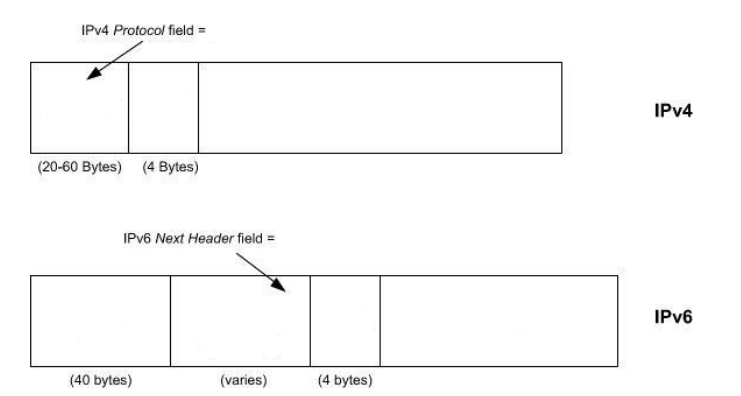
\includegraphics[scale=0.5]{icmp1}
		\caption{Generischer Aufbau eines ICMP-Pakets für IPv4 und IPv6.}
		\label{icmp1}
		\end{figure}
		\item Welche Nachrichtentypen werden für den Ping-Messages genutzt? Wo sind die Nachrichtentypen zu finden?
		\item Skizzieren sie mithilfe von Abb.\ref{icmp2} die ICMP-Nachricht und welche Informationen Wireshark ihnen liefert.
		\begin{figure}[H]
		\centering
		\includegraphics[scale=0.5]{icmp2}
		\caption{Nutzlast eines ICMP-Pakets.}
		\label{icmp2}
		\end{figure}
	\end{enumerate}
	\item Starten sie eine Routenverfolgung via \emph{traceroute} auf eine beliebige Adresse. Verfolgen sie dabei die Ausgabe auf der Konsole und Wireshark (Filtern sie in Wireshark entsprechend). Spiegeln sich die Einträge in Wireshark mit denen auf der Kommandozeile?
	\item Welche ICMP-Nachrichten wurden hier verwendet?
	\item Erläutern sie die genaue Routenverfolgung mithilfe der ICMP-Nachrichten. Welches Feld wird hier genutzt um jeden Hop \enquote{verfolgen} zu können?
	\item Überlegen sie sich zunächst anhand Ihrer Recherche was \emph{traceroute} in etwa ausgeben müsste, wenn sie auf der VM eine Route von einem Rechner $A$ zu einem Rechner $B$ verfolgen würden. Wobei beide Rechner zu unterschiedlichen LANs gehören. 
	\item Nutzen Sie anschließend \emph{traceroute} um sich die Router zwischen zwei VMs anzeigen zu lassen. Stimmen Ihre theoretische Überlegungen mit denen von \emph{traceroute} überein? Falls nicht, sollten Sie analysieren woran dies liegen könnte.
\end{enumerate}

\begin{center}
\Large{\textbf{Aufgabe D - Bestimmung des physischen Rechners zu einer IP-Adresse -- ARP}}
\end{center}\vskip0.25in
Sie haben bereits theoretisch recherchiert, wie die Zuordnung von physischer Adresse zu einer IP-Adresse vonstatten geht. Im Folgenden sollen sie herausfinden, ob die Auflösung von IP-Adresse auf physische Adresse wirklich analog zu ihren theoretischen Recherchen abläuft.
\begin{enumerate}
	\item Um einen ARP-Request auszulösen können sie das Werkzeug \emph{arp} nutzen. Lesen sie in der \emph{man}-Page:
	\begin{itemize}
		\item Wie können sie sich ihre MAC-Adresse und Interface anzeigen lassen?
		\item Wie können sie sich den ARP-Table ausgeben lassen?
		\item Wie leeren sie den ARP-Cache?
	\end{itemize}
	\item Finden sie mithilfe Wiresharks heraus, wie die Adressauflösung funktioniert.
		\begin{enumerate}
			\item Starten sie Wireshark und stellen sie das korrekte Interface ein.
			\item Leeren sie zunächst den ARP-Cache.
			\item Pingen sie nun einen Rechner an, den sie vorhin noch nicht \enquote{angepingt} haben. Die dafür ausgetauschten Pakete werden nun \enquote{gesnifft}.
			\item Beenden sie das Mitschneiden des Netzwerksverkehrs und setzen sie als Filtern die MAC-Adresse ihres Adapters.
			\item Versuchen sie über den Mitschnitt herauszufinden, wie die Bestimmung des zugehörigen Netzadapters und die MAC-Adresse erfolgt.
		\end{enumerate}
	\item Damit ihr Rechner nicht jedes mal eine Auflösung veranlassen muss, werden die ARP-Informationen lokal in einem Cache zwischengespeichert (\enquote{cached}).
\begin{enumerate}
	\item Lassen sie sich Ihren aktuellen ARP-Cache anzeigen. Welche Informationen können sie diesem entnehmen?
	\item Schauen sie kurz nach, wie lange der ARP-Cache Einträge vorhält.
	\item Lassen sie zwei VMs die IP-Adressen tauschen. Dies sollte möglichst schnell umgesetzt werden!
	\item Versuchen sie nun durch eine dritte VM eine \enquote{alte} IP-Adresse zu erreichen. Werden die Daten an den richtigen Knoten übermittelt?
	\item Verfolgen sie die Datenübermittlung per Wireshark mit.
\end{enumerate}
\end{enumerate}

\begin{center}\Large{\textbf{Aufgabe E -- TCP: 3-Way-Handshake}}\end{center}\vskip0.2in
Nachdem sie sich bereits theoretisch mit dem 3-Way-Handshake auseinandergesetzt haben, sollen sie nun schauen, ob der TCP-Handshake tatsächlich wie theoretisch beschrieben arbeitet.
\begin{enumerate}
	\item Überlegen sie sich eine Anfragen an eine Website (dies sollte TCP nutzen, etwa durch ein HTTP-Request!), die sie noch nicht von der VM aus getätigt haben.
	\item Starten sie Wireshark, richten sie Interface und Protokolltype ein. Filtern sie nur auf eine speziellen Request!
	\item Lösen sie den Handshake durch aufrufen der Website (oder Ressource) aus, während Wireshark den Netzverkehr mitschneidet.
	\item Analysieren sie den 3-Way-Handshake!
	\item Zum Vergleich: Analysieren Sie ihren Mitschnitt mit folgender Aufzeichnung: \url{https://wiki.wireshark.org/TCP_3_way_handshaking?action=AttachFile&do=view&target=3-way+handshake.pcap}
\end{enumerate}

\begin{center}
\Large{\textbf{Fakultative Aufgabe - Packet Analysis}}
\end{center}\vskip0.25in

Im Moodle-Kurs liegt eine Zip-Datei \path{network_packets.zip}. Diese enthält verschiedene Dateien die sie auf verschiedene Arten in Wireshark öffnen können. Sie sollen diese Pakete analysieren. Teilweise sind in diesen Paketen Passwörter und Zugangsdaten zu finden, in einigen Fällen können ganze Nachrichten oder Geräteinformationen gefunden werden.
\begin{enumerate}
	\item Die Datei \path{ftp.pcap} ist eine FTP-Session mit Passwort Authentifizierung. Finden sie das Paket sowie Passwort.
	\item Die Datei \path{telnet.pcap} ist eine Telnet-Session mit Passwort Authentifizierung. Finden sie das Paket sowie Passwort.
	\item Die Datei \path{twitter.pcap} ist eine Twitter-Session welche die Authentifizierung enthält. Finden sie heraus, wie diese umgesetzt wurde und finden sie das Passwort.
	\item Die Datei \path{bt.bin} für die Authentisierung von Bluetooth-Geräten gedacht. Im wesentlichen benötigen sie die MAC-Adresse des Gerätes und den Gerätenamen. Beides ist in der Datei enthalten. Die Authentisierung erfolgt die Hashing mit SHA1 (eine kryptografische Hashfunktion \footnote{Mehr dazu demnächst. SHA1 gilt seit Jahren als unsicher!}). Finden sie das Tupel aus MAC-Adresse und Gerätenamen heraus und lassen Sie die SHA1 Funktion darüber laufen.
	\begin{lstlisting}[style=Bash, language=Bash]
echo "XXXXXXXXXXXXXXXXXXX" | sha1sum
\end{lstlisting}
\end{enumerate}


\end{document}